\section{4. Modulaci\'on de se\~nal con FM}
La modulci\'on FM consiste en utilizar una señal modulante para variar la frecuencia de la señal portandora alrededor de la frecuencia portadora en un rango espec\'ifico. Puede definirse al igual que en modulaci\'on AM un coeficiente de modulaci\'on , el cual representa la desviaci\'on de frecuencia m\'axima como multiplo de la m\'axima frecuencia de la moduladora. Para este ejercicio se repitieron los puntos $b$, $c$ y $d$ del inciso anterior para una modulaci\'on FM. 


\subsection{Mediciones}
A continuaci\'on se dejan los espectros obtenidos:


\begin{figure}[H]
    \centering
    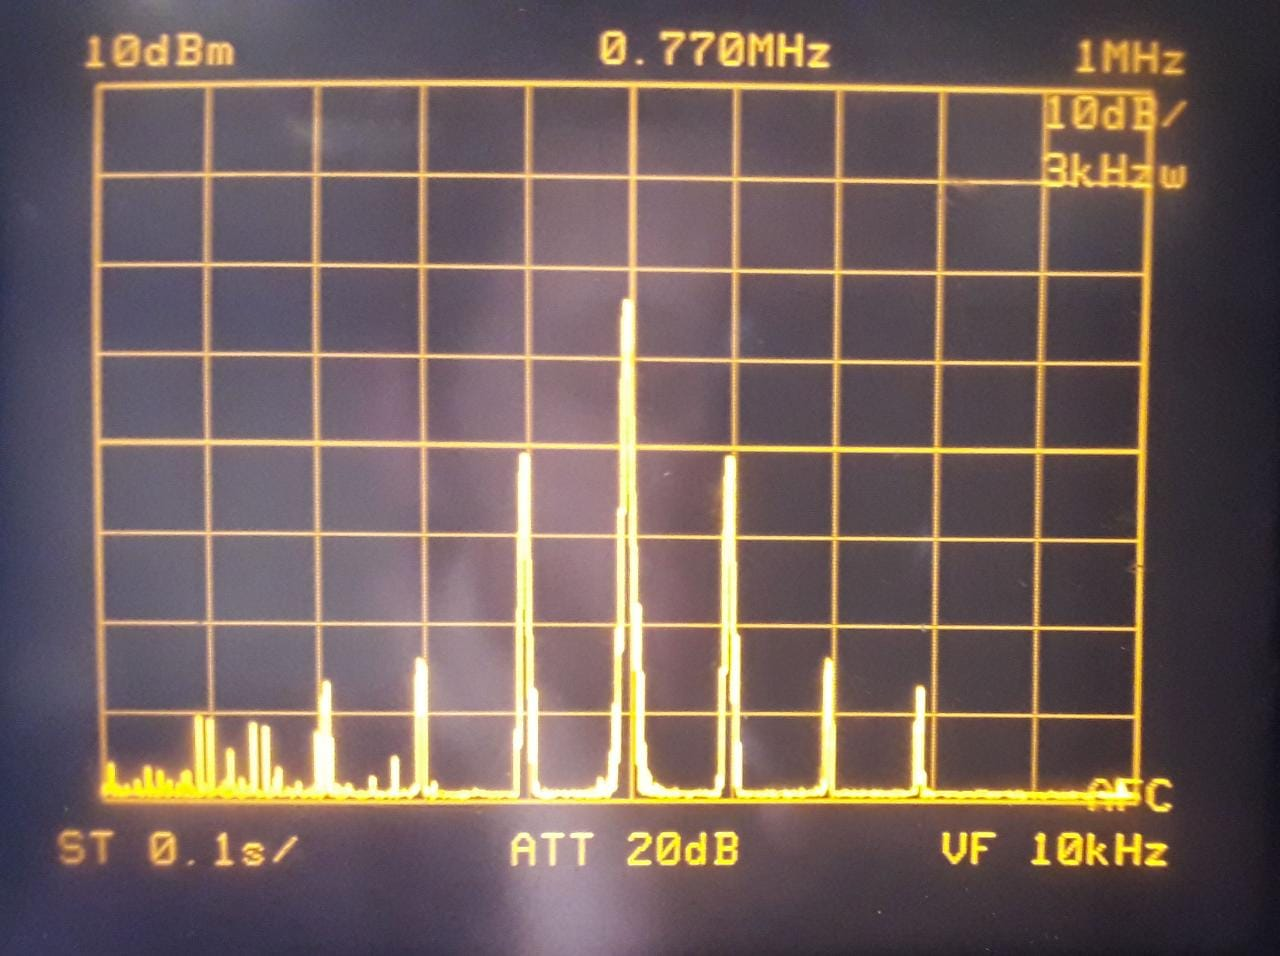
\includegraphics[scale=0.3]{Recursos/Ej4_senoidal.jpeg}
    \caption{Espectro señal senoidal con $m = 0.5$}
\end{figure}\label{fig:espectro1}

\begin{figure}[H]
    \centering
    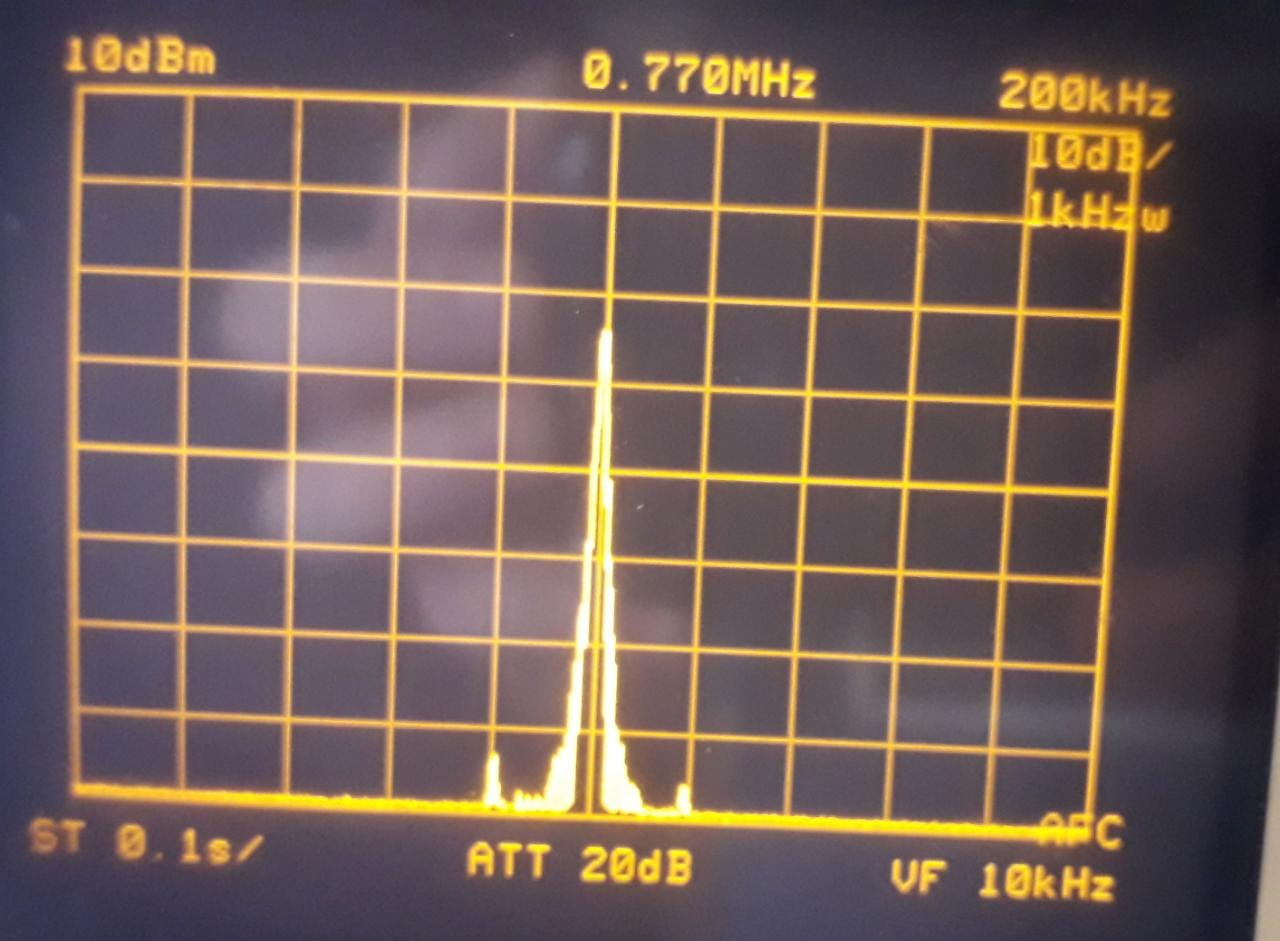
\includegraphics[scale=0.3]{Recursos/Ej4_senoidal_800K.jpeg}
    \caption{Espectro señal senoidal con frecuencia portadora}
\end{figure}

\begin{figure}[H]
    \centering
    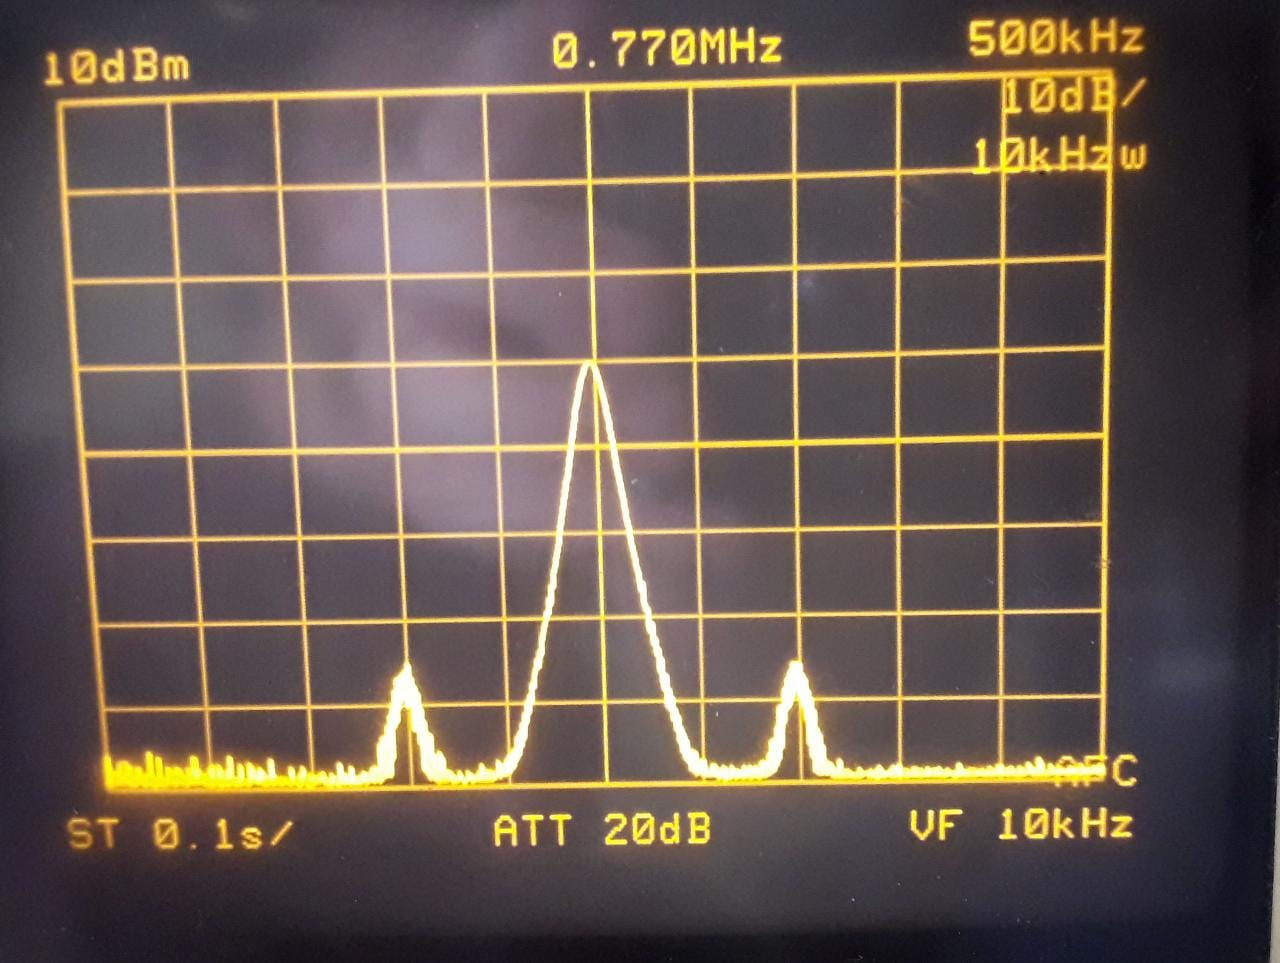
\includegraphics[scale=0.3]{Recursos/Ej4_triangular_m1.jpeg}
    \caption{Espectro señal triangular con $m = 1$}
\end{figure}


\subsection{An\'alisis de los resultados}

Debido a que en la modulación FM se hace variar la frecuencia de la portadora se esperaría ver ese comportamiento reflejado en forma de armónicos en el analizador de espectros. En la figura \ref{fig:espectro1} se ve claramente lo anterior, en el centro, nuevamente desvíada en $30kHz$ está la frecuencia fundamental, y alrededor de ella se ven 3 pares de armónicos distanciados de manera proporcional, por lo que se cumple la hipótesis incial de modulación FM. Para el caso en el que las frecuencias de las dos señales son iguales ocurre lo mismo que en el ejercicio anterior, y no hya armónicos presentes. Para la triangular, la explicación es análoga al ejercicio 3.

